\chapter{Version Control}
	Door middel van version control kunnen meerdere ontwikkelaars aan dezelfde software werken.
	Tijdens JEA6 zal Git (GitHub) gebruikt worden voor version control. Er is hiervoor gekozen omdat hiermee reeds de meeste ervaring is opgedaan.
	
	\begin{figure}[H]
			\includegraphics[width=0.50\textwidth]{images/configuredBranches.png}
			\caption{Overzicht van default branch en protected branches}
			\label{fig:ConfiguredBranches}
	\end{figure}
	
	\section{Branches}
	Voor de repository waar de code van het vak JEA6 wordt bijgehouden, zijn verschillende branches aangemaakt. Wat het nu is van deze verschillende branches, staat in de volgende alinea's uitgelegd.
	
	\begin{figure}[H]
			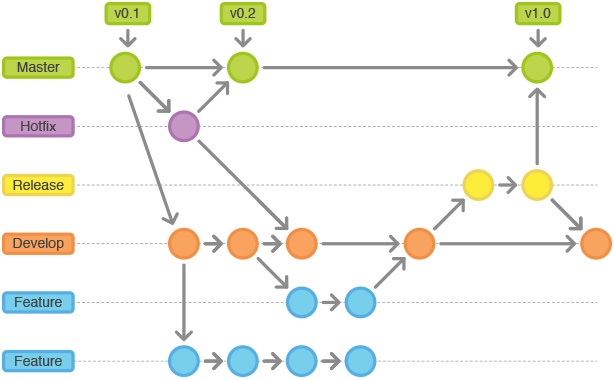
\includegraphics[width=0.75\textwidth]{images/BranchScheme.png}
			\caption{Schematisch overzicht van de branches}
			\label{fig:BranchScheme}
	\end{figure}
	
	\subsection{Master}
	De code die beschikbaar is in de master-branch, is de code van de software versie die in productie gebruikt wordt. Nieuwe functies of bug fixes mogen dan ook niet rechtstreeks naar deze branch gecommit worden.
	Deze branch is tevens protected. Dit wilt zeggen dat vanuit een git programma (UI of CLI) niet rechtstreeks naar deze branch gecommit kan worden. Dit zorgt ervoor dat een ontwikkelaar niet per ongeluk naar deze branch kan committen.
	
	
	\begin{figure}[H]
	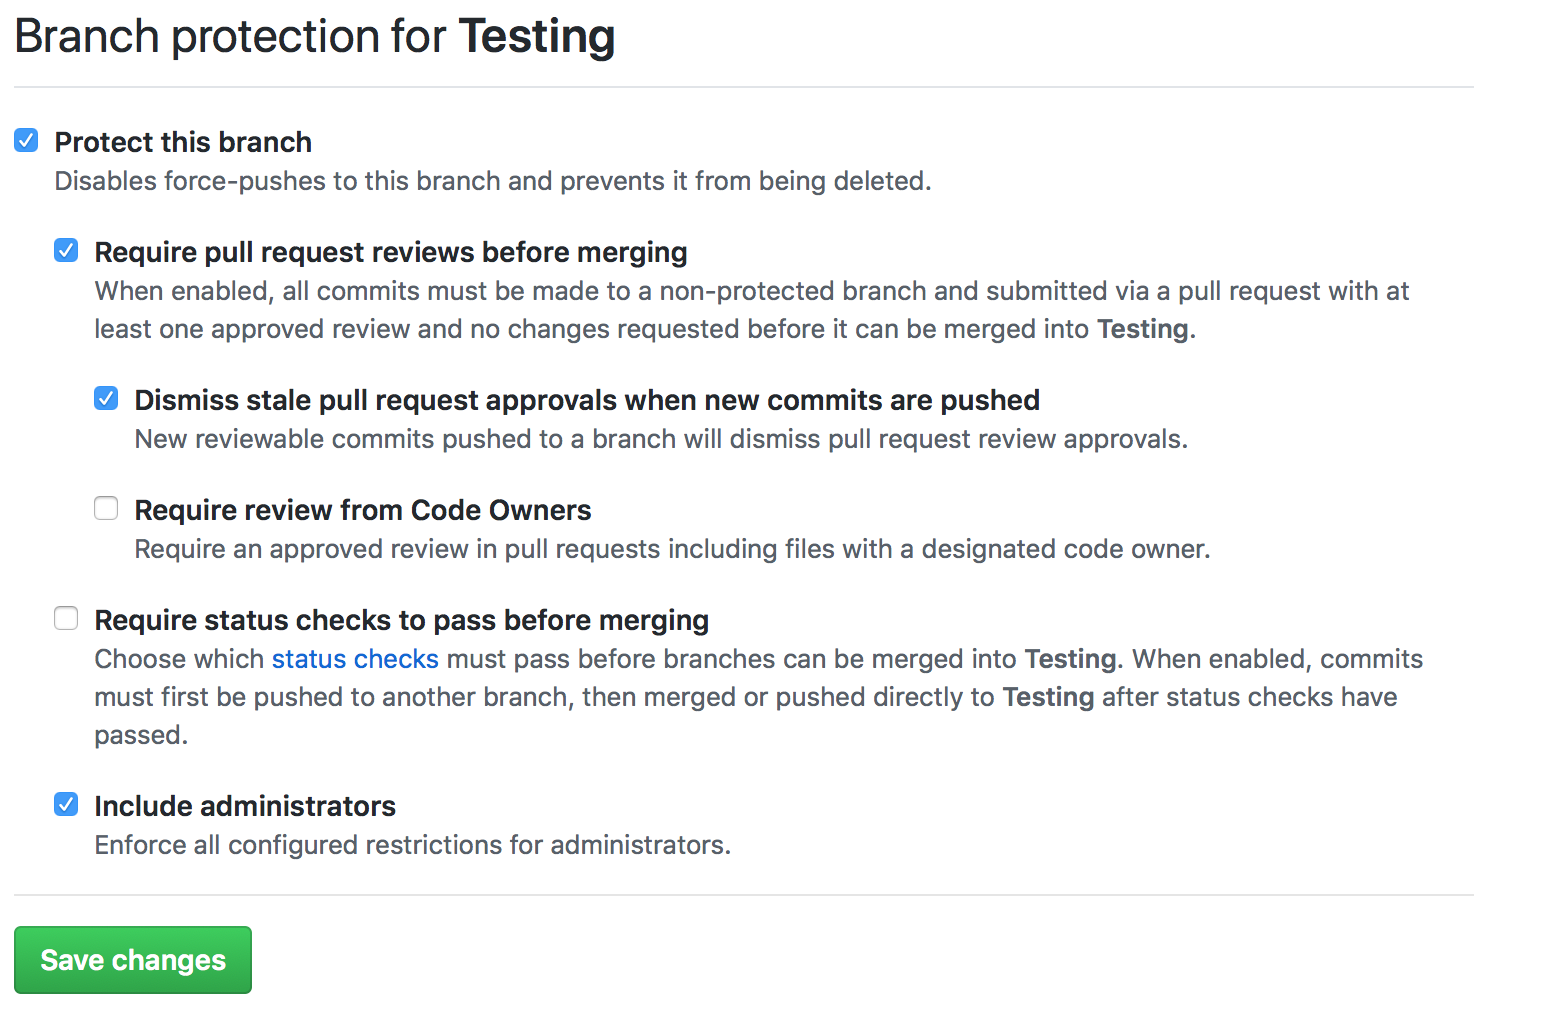
\includegraphics[width=0.5\textwidth]{images/BranchProtectionSetup.png}
	\caption{Overzicht van protectie wat ingesteld is op branch}
	\label{fig:BranchProtectionSetup}
	\end{figure}

	\subsection{Hotfix}
	
	\subsection{Testing}
	De Testing-branch zal gebruikt worden om nieuwe functionaliteit die ontwikkeld zijn in de development branch te testen. Wanneer de functionaliteit in de testing branch geaccepteerd wordt, zal deze worden doorgezet naar de master branch zodat de verbeteringen en/of nieuwe wijzigingen beschikbaar zijn voor alle gebruikers op de productie omgeving
	De Testing-branch heeft dezelfde setup als de Master-branch. Dit wilt zeggen dat het op deze branch ook niet mogelijk is om rechtstreeks code te committen.
	
	De testing omgeving die gebruikt wordt om de code van de testing branch beschikbaar te stellen, kan tevens gebruikt worden door testers om nieuwe functionaliteit of verbeteringen te testen. Daarnaast kan de release manager akkoord geven op de versie die in deze omgeving staat, waardoor deze verplaatst zal worden naar de productie omgeving
	\subsection{Development}
	
	De Development-branch bevat nieuwe functionaliteit of verbeteringen wat ontwikkeld zijn. Deze branch is vrij toegangkelijk voor de ontwikkelaar om eventueel kleine(re) verbeteringen door te voeren.	
	Het is als nog de bedoeling dat nieuwe functionaliteit niet rechtstreeks op deze branch wordt gecommit. Mocht een ontwikkelaar nieuwe functionaliteit of grotere verbeteringen willen ontwikkelen, kan hiervoor een zogenaamde Feature-branch worden aangemaakt. Meer informatie hierover is in de volgende alinea te lezen
	
	\subsection{Features}
	De Features-branch is geen branch die direct aangemaakt is op Github. Dit komt doordat "Features"\ een overkoepelende term is. Wanneer een ontwikkelaar nieuwe functionaliteit of verbeteringen wilt ontwikkelen, dan zal hiervoor een nieuwe branch moeten worden aangemaakt, bijvoorbeeld "Dev-exampleFeature". Aan de hand van de prefix "Dev-" weet iedereen dat dit een branch betreft waar nieuwe functionaliteit of verbeteringen op worden ontwikkeld. Het gedeelte achter de prefix moet dan ook beschrijven aan welke functionaliteit of verbeteringen worden gewerkt.
	
	
	Wanneer de ontwikkelaar het implementeren heeft voltooid, zal dit eerst getest moeten worden op zijn eigen, lokale omgeving. Wanneer die nieuwe functionaliteit werkt met de rest van de ontwikkelde software, kan de ontwikkelaar zijn branch, bijvoorbeeld "Dev-exampleFeature"\ gaan samenvoegen met de Development-branch. Hiervoor maakt de ontwikkelaar een merge request aan wat ervoor zorgt dat de nieuwe code wordt samengevoegd op de Development-branch.
	
	\subsection{Bugfix/Patches}